% GNUPLOT: LaTeX picture with Postscript
\begingroup
  \makeatletter
  \providecommand\color[2][]{%
    \GenericError{(gnuplot) \space\space\space\@spaces}{%
      Package color not loaded in conjunction with
      terminal option `colourtext'%
    }{See the gnuplot documentation for explanation.%
    }{Either use 'blacktext' in gnuplot or load the package
      color.sty in LaTeX.}%
    \renewcommand\color[2][]{}%
  }%
  \providecommand\includegraphics[2][]{%
    \GenericError{(gnuplot) \space\space\space\@spaces}{%
      Package graphicx or graphics not loaded%
    }{See the gnuplot documentation for explanation.%
    }{The gnuplot epslatex terminal needs graphicx.sty or graphics.sty.}%
    \renewcommand\includegraphics[2][]{}%
  }%
  \providecommand\rotatebox[2]{#2}%
  \@ifundefined{ifGPcolor}{%
    \newif\ifGPcolor
    \GPcolortrue
  }{}%
  \@ifundefined{ifGPblacktext}{%
    \newif\ifGPblacktext
    \GPblacktexttrue
  }{}%
  % define a \g@addto@macro without @ in the name:
  \let\gplgaddtomacro\g@addto@macro
  % define empty templates for all commands taking text:
  \gdef\gplbacktext{}%
  \gdef\gplfronttext{}%
  \makeatother
  \ifGPblacktext
    % no textcolor at all
    \def\colorrgb#1{}%
    \def\colorgray#1{}%
  \else
    % gray or color?
    \ifGPcolor
      \def\colorrgb#1{\color[rgb]{#1}}%
      \def\colorgray#1{\color[gray]{#1}}%
      \expandafter\def\csname LTw\endcsname{\color{white}}%
      \expandafter\def\csname LTb\endcsname{\color{black}}%
      \expandafter\def\csname LTa\endcsname{\color{black}}%
      \expandafter\def\csname LT0\endcsname{\color[rgb]{1,0,0}}%
      \expandafter\def\csname LT1\endcsname{\color[rgb]{0,1,0}}%
      \expandafter\def\csname LT2\endcsname{\color[rgb]{0,0,1}}%
      \expandafter\def\csname LT3\endcsname{\color[rgb]{1,0,1}}%
      \expandafter\def\csname LT4\endcsname{\color[rgb]{0,1,1}}%
      \expandafter\def\csname LT5\endcsname{\color[rgb]{1,1,0}}%
      \expandafter\def\csname LT6\endcsname{\color[rgb]{0,0,0}}%
      \expandafter\def\csname LT7\endcsname{\color[rgb]{1,0.3,0}}%
      \expandafter\def\csname LT8\endcsname{\color[rgb]{0.5,0.5,0.5}}%
    \else
      % gray
      \def\colorrgb#1{\color{black}}%
      \def\colorgray#1{\color[gray]{#1}}%
      \expandafter\def\csname LTw\endcsname{\color{white}}%
      \expandafter\def\csname LTb\endcsname{\color{black}}%
      \expandafter\def\csname LTa\endcsname{\color{black}}%
      \expandafter\def\csname LT0\endcsname{\color{black}}%
      \expandafter\def\csname LT1\endcsname{\color{black}}%
      \expandafter\def\csname LT2\endcsname{\color{black}}%
      \expandafter\def\csname LT3\endcsname{\color{black}}%
      \expandafter\def\csname LT4\endcsname{\color{black}}%
      \expandafter\def\csname LT5\endcsname{\color{black}}%
      \expandafter\def\csname LT6\endcsname{\color{black}}%
      \expandafter\def\csname LT7\endcsname{\color{black}}%
      \expandafter\def\csname LT8\endcsname{\color{black}}%
    \fi
  \fi
    \setlength{\unitlength}{0.0500bp}%
    \ifx\gptboxheight\undefined%
      \newlength{\gptboxheight}%
      \newlength{\gptboxwidth}%
      \newsavebox{\gptboxtext}%
    \fi%
    \setlength{\fboxrule}{0.5pt}%
    \setlength{\fboxsep}{1pt}%
\begin{picture}(5000.00,5142.00)%
    \gplgaddtomacro\gplbacktext{%
      \csname LTb\endcsname%
      \put(1118,3780){\makebox(0,0)[r]{\strut{}$280$}}%
      \put(1118,4143){\makebox(0,0)[r]{\strut{}$320$}}%
      \put(1118,4506){\makebox(0,0)[r]{\strut{}$360$}}%
      \put(1118,4869){\makebox(0,0)[r]{\strut{}$400$}}%
      \put(1250,3379){\makebox(0,0){\strut{} }}%
      \put(1714,3379){\makebox(0,0){\strut{} }}%
      \put(2178,3379){\makebox(0,0){\strut{} }}%
      \put(2642,3379){\makebox(0,0){\strut{} }}%
      \put(3107,3379){\makebox(0,0){\strut{} }}%
      \put(3571,3379){\makebox(0,0){\strut{} }}%
      \put(4035,3379){\makebox(0,0){\strut{} }}%
      \put(4499,3379){\makebox(0,0){\strut{} }}%
      \put(1347,4971){\makebox(0,0)[l]{\strut{}a)}}%
    }%
    \gplgaddtomacro\gplfronttext{%
      \csname LTb\endcsname%
      \put(480,4370){\rotatebox{-270}{\makebox(0,0){\strut{}$\left< R^2\right>  \,[\SI{}{\square\angstrom}]$}}}%
    }%
    \gplgaddtomacro\gplbacktext{%
      \csname LTb\endcsname%
      \put(1118,2144){\makebox(0,0)[r]{\strut{}$0.3$}}%
      \put(1118,2585){\makebox(0,0)[r]{\strut{}$0.4$}}%
      \put(1118,3025){\makebox(0,0)[r]{\strut{}$0.5$}}%
      \put(1118,3466){\makebox(0,0)[r]{\strut{}$0.6$}}%
      \put(1250,1836){\makebox(0,0){\strut{} }}%
      \put(1714,1836){\makebox(0,0){\strut{} }}%
      \put(2178,1836){\makebox(0,0){\strut{} }}%
      \put(2642,1836){\makebox(0,0){\strut{} }}%
      \put(3107,1836){\makebox(0,0){\strut{} }}%
      \put(3571,1836){\makebox(0,0){\strut{} }}%
      \put(4035,1836){\makebox(0,0){\strut{} }}%
      \put(4499,1836){\makebox(0,0){\strut{} }}%
      \put(1347,3428){\makebox(0,0)[l]{\strut{}b)}}%
    }%
    \gplgaddtomacro\gplfronttext{%
      \csname LTb\endcsname%
      \put(480,2827){\rotatebox{-270}{\makebox(0,0){\strut{}$\left<P_{2}^{xz}\right>$}}}%
    }%
    \gplgaddtomacro\gplbacktext{%
      \csname LTb\endcsname%
      \put(1118,514){\makebox(0,0)[r]{\strut{}$60$}}%
      \put(1118,977){\makebox(0,0)[r]{\strut{}$90$}}%
      \put(1118,1439){\makebox(0,0)[r]{\strut{}$120$}}%
      \put(1118,1902){\makebox(0,0)[r]{\strut{}$150$}}%
      \put(1250,294){\makebox(0,0){\strut{}0}}%
      \put(1714,294){\makebox(0,0){\strut{}100}}%
      \put(2178,294){\makebox(0,0){\strut{}200}}%
      \put(2642,294){\makebox(0,0){\strut{}300}}%
      \put(3107,294){\makebox(0,0){\strut{}400}}%
      \put(3571,294){\makebox(0,0){\strut{}500}}%
      \put(4035,294){\makebox(0,0){\strut{}600}}%
      \put(4499,294){\makebox(0,0){\strut{}700}}%
      \put(1347,1886){\makebox(0,0)[l]{\strut{}c)}}%
    }%
    \gplgaddtomacro\gplfronttext{%
      \csname LTb\endcsname%
      \put(480,1285){\rotatebox{-270}{\makebox(0,0){\strut{}$F_L \, [\SI{}{\mega\pascal}]$}}}%
      \put(2874,-36){\makebox(0,0){\strut{}Distance [\SI{}{\nano\meter}]}}%
      \csname LTb\endcsname%
      \put(4040,1883){\makebox(0,0)[r]{\strut{}\SI{10}{\meter\per\second}}}%
      \csname LTb\endcsname%
      \put(4040,1663){\makebox(0,0)[r]{\strut{}\SI{20}{\meter\per\second}}}%
      \csname LTb\endcsname%
      \put(4040,1443){\makebox(0,0)[r]{\strut{}\SI{50}{\meter\per\second}}}%
      \csname LTb\endcsname%
      \put(4040,1223){\makebox(0,0)[r]{\strut{}\SI{100}{\meter\per\second}}}%
    }%
    \gplbacktext
    \put(0,0){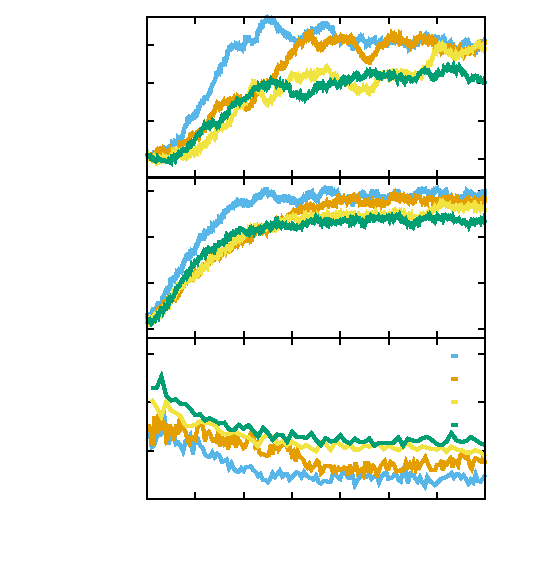
\includegraphics{main-gnuplottex-fig1}}%
    \gplfronttext
  \end{picture}%
\endgroup
